\chapter[Spatial proteomic for mapping spatial cell types and identifying interactions across tissue]{Spatial proteomic for mapping spatial cell types and identifying interactions across tissue}
\label{Chap:3}	%CREATE YOUR OWN LABEL.
\pagestyle{headings}
\section{Introduction}
\label{Sec:3.1_intro}
%CREATE YOUR OWN LABEL.
While the number of gene markers can be profiled using cutting edge spatial transcriptomic is growing rapidly, i.e. Visium (10X Genomic),  Stereo-Seq (BGI), it is important to note that not all RNA expression are highly correlated with translated protein expression level. Therefore, spatial proteomic is an important complementary tools to uncover the complex heterogeneity of cancerous cell and their intercellullar connection with other cells. Advances in multiplexed tissue imaging enables analysis of up to hundreds of proteins in thousands of cells in a single experiments. Protein profile of a tissue has been analysed, it cam provide an additional layer of connection from cells to environment context and biological processes. 

For this chapter, I focused more on quantifying the cellular structures and the cross-talk between cell types in cancer tissues using two spatial proteomics technologies: Vectra Polaris in skin cancer and Imaging Mass Cytometry (IMC) \cite{giesen2014IMC} in colorectal cancer (Table: \ref{table:DataInfor}). The former dataset I was working on  consists of 6 whole slide skin cancer tissues which were scanned by highly multiplex Polaris technologies. Each slide was processed with a panel of 6 proteins CD8, PD-L1, PD-1, FoxP3, CD68, Pan-cytokeratin (PanCK) and DAPI for nuclei staining. Meanwhile for the colorectal cancer, the experiment was designed to use IMC technology to capture the protein expression of a panel of 15 protein markers from 51 patients with stage 3 colon adenocarcinoma. The IMC protein panel consists of structural markers  Epithelial (E-cadherin, Keratin), Fibroblast (collagen), cell proliferative marker (Ki-67) and several immune markers including for T-cells (CD8), regulatory T cells (FoxP3), macrophages (CD68+), B cells (CD20+), etc. Unlike Polaris technology, IMC performs tissue scanning at multiple regions of interest (ROIs) selected from whole slide tissue. Although, the two input datasets captured different antibody panels as well as different cancer types, they both produce protein expression data at subcellular resolution retaining  a wealth of spatial information.    

\begin{table}[ht]
\centering
\caption{Summary of data specification}
\begin{tabular}{||P{7cm} || P{3cm} || P{3cm} ||} 
 \hline
 Specifications & Colorectal Cancer Samples & Skin Cancer Samples   \\ [0.33ex] 
 \hline\hline
 Number of patients & 52 & 3   \\ 
 \hline
 Number of Markers & 16 markers & 6 markers  \\ 
 \hline
 Number of images & 126 ROIs &  6 whole slides \\
 \hline
 Diagnosis & Stage 3 adenocarcinoma & Basal Cell Carcinoma  \\ [1ex] 
 \hline
\end{tabular}
\label{table:DataInfor}
\end{table}


% ***************************************************
\section{Cell type identification and cell communities detection methods}
\label{Sec:3.2_CCC_ST}	%CREATE YOUR OWN LABEL.
\subsection{Adapting cell type identification from existing scRNA-seq methods}
Before any CCC analysis, a key step  to make use of sub-cellular spatial proteomic information is to perform cell segmentation and cell type identification. Depending on the size of the whole slide tissue, Polaris imaging in our skin cancer dataset captured around $40000\sim 79000$ cells per tissue with fluorescence values quantified for each marker. To employ the current established cell clustering and annotation, the Polaris imaging was transformed into a non-imaging-based data through cell segmentation (Figure: \ref{fig:Polaris_skin_cancer_cell_iden}A,B) \cite{hickey2021strategies}. More specifically, cell segmentation was carried out throughout the tissue using a deep learning model called stardist \cite{schmidt2018cell}, which eventually turned every nuclei in the DAPI channel into a list of cell objects. For each cell object, the protein signal intensity was normalised to the mean DAPI intensity within cell boundary and assigned to expression level of that protein to the cell (Figure: \ref{fig:Polaris_skin_cancer_cell_iden}B-D). In order to remove the artificially high background from fluorescent intensities (outliers), $95^{th}$ percentile was used to cap the maximum value of each marker (Figure: \ref{fig:Polaris_skin_cancer_cell_iden}D). After the preprocessing of proteomics data, a standard cell type clustering was applied using a common single-cell processing pipeline, scanpy \cite{wolf2018scanpy}. Based on the panel of 6 proteins, we were able to identify several major epithelial (PanCK+), inmate immune cells (CD68+) and adaptive immune cells (CD8+, FoxP3+) (Fig: \ref{fig:skin_cancer_polaris}A). Among all the clusters detected by the scanpy pipeline (leiden clustering), those cells with very low expression of all the proteins in the panel were classified as unidentified and removed from downstream analysis. The cell identifications were eventually plotted back to the original spatial context for validation.  

Similarly, for our IMC imaging dataset of colorectal cancer, the first analysis steps are cell segmentation and cell clustering. The key differences between Polaris and IMC are the resolution of the images generated by each technology. While every pixel in the Polaris image captures $0.49 \mu m$ in the real tissue, the specification in IMC is $1$pixel representing $1\mu m$. IMC generated discrete signal (counts of heavy metal molecules) which requires a specialised cell segmentation method. Currently, the IMC segmentation pipeline is being adapted from a pipeline by Bodenmiller Group, one of the founders of the technology (\href{https://github.com/BodenmillerGroup/ImcSegmentationPipeline/blob/development/scripts/imc_preprocessing.ipynb}{Github IMC preprocessing pipeline}. In short, the raw IMC data (.mcd file) are converted into a standard image format with multiple channels and each channel represent the expression of a staining marker. Because the signal intensity in IMC has lower resolution yet noisier than in Polaris, we manually built a segmentation model to assign pixels to either cell nuclei, cytoplasm or background using two steps with CellProfiler and Ilastik \cite{carpenter2006cellprofiler, berg2019ilastik}. Since IMC imaging data were generated only for selected ROI, not the whole tissue, the number of cells in this project is significantly lower than that in the skin cancer project, ranging from $200$ to $1600$ cells per ROI (~3 ROIs/sample) . After the cell segmentation, similar data preprocessing is applied to map signals to a list of cell objects. Cellular data was then clipped to remove outliers. For cell type annotation, major structural cell types could be identified with high confidence such as Epithelial or Cancer (E-cadherin and Keratin), Fibroblast and Stromal (Collagen, SM-actin). We were also able to annotate other adaptive like B-cells (CD20), CD8 T-cells (CD8), T-reg cells (CD4, FoxP3) and inmate immune cell type Macrophages (CD68) (Fig:\ref{fig:colorectal_cancer_IMC}A). Finally, for validation, we compared the IMC-identified cell types against pathologist annotation. Through a process called image registration, we were able to align the IMC image to the adjacent section of H\&E image which was annotated with some cell types by pathologist (Fig:\ref{fig:colorectal_cancer_IMC}B). Since our computational results matched well with manual annotation this gave us confidence in our cell segmentation and clustering approaches before proceeding towards the CCC analyses. 

\begin{figure}[htp]
    \centering
    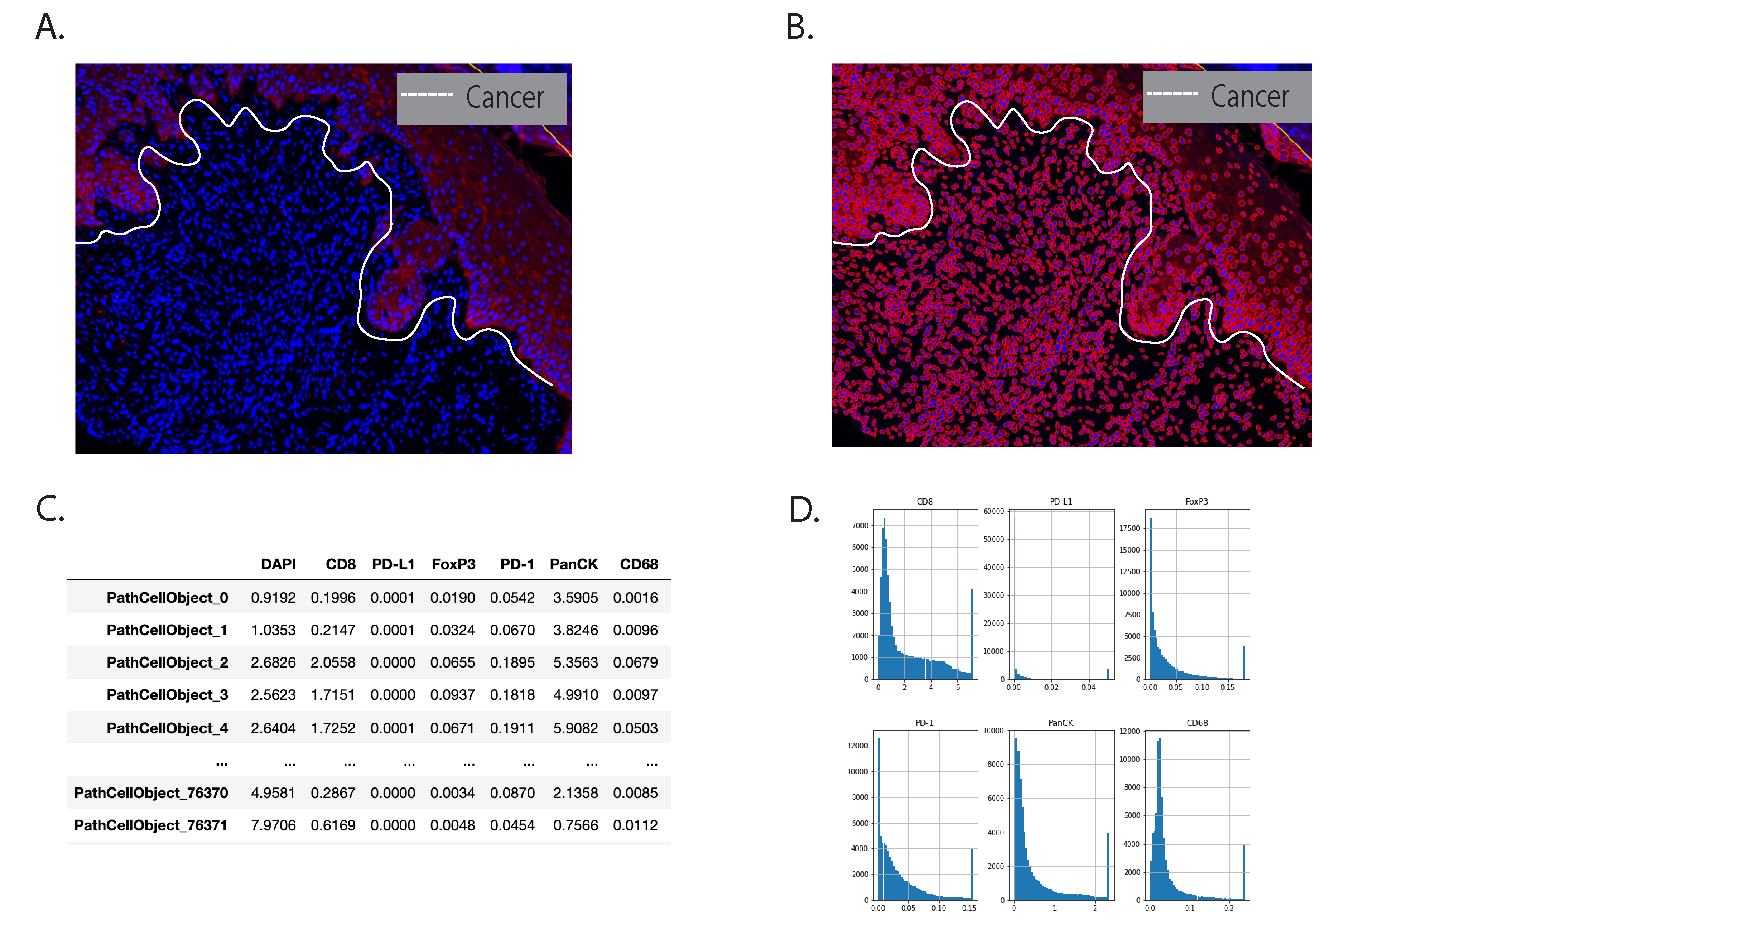
\includegraphics[width=\columnwidth]{Chapter3/Figures/Cell_identification_skin_cancer-01.png}
    \caption{Schematic of data preprocessing for cell type annotation. (A) A zoomed in image of cell the nuclei representation in DAPI channel (dark blue) and cytokeratin marker expression (PanCK in red) for epithelial cell marker. The annotation line in white separates the cancer lesions of the skin from the lower layer. (B) Detection and segmentation of cells from the image using the nuclei channel. (C) The conversion of imaging-based data to single-cell-based data by measuring the level signal each cell expresses within the cell boundary. (D) Histograms of the expression level of each protein in the panels across all the detection cells}
    \label{fig:Polaris_skin_cancer_cell_iden}
\end{figure}

\subsection{Detecting cell communities based on cells spatial organisation}
There are already a few computational methods that used scRNA-seq to infer the CCC i.e. CellChat \cite{jin2021CellChat}, CellPhoneDB \cite{efremova2020cellphonedb} or NicheNet \cite{browaeys2020nichenet}. However, they are all unable to address the spatial constraints of interactions. With scRNA-seq data, the limited insights into the spatial location of the RNA molecules within a cell and the organization of cells in a tissue prevent the CCC inference from reaching its potential. To address this, the development of higher multiplexed histological techniques for capturing transcriptomic or/and proteomic information at subcellular resolution, e.g. co-detection by imaging (CODEX) \cite{goltsev2018CODEX} or IMC from Hyperion, facilitated the integration of spatial information into CCC inference. 

Given the growing number of spatially resolved transcriptomic and proteomic technologies, the current available analysis strategies to process these high dimensional data have not yet exploited the full potential of spatial information. In short, spatially resolved CCC analysis can be categorised into two main groups. The first approach considers each cell as a point in Cartesian coordinate system and assesses the changes in the spatial co-localisation between pairs of cell types at distances \cite{arnol2019modeling,schurch2020coordinated}. Meanwhile, the second path considers only the interactions of each cell and its intermediate adjacent cells within a short proximity from the cell membrane. It is sufficient to measure cell-cell interaction through gap junction or paracrine signalling. The pairwise interaction of two cell types is then grouped by cell phenotypes and compared to randomised label of cells to determine significance of interactions  \cite{schapiro2017histocat}.  In the following sections, I will go deeper into the advantages and disadvantages of each approach and about how I applied them throughout my second-year projects.    

PD1 has been extensively studied and identified as immune inhibitor for skin cancer cell growth\cite{ishida1992induced,  tsai2014pd}. In the first project using skin cancer as the model to study, we were interested in finding and validating the immune-cancer cell interactions pairing the ligand-receptor PD-L1 and PD1 through a series of spatial analysis methods. On the other hand, we sought to find the pattern of intercellular architecture in colorectal cancer and the correlation between alterations in CCC and the prognosis for the patients. Once the cells were clustered and annotated appropriately, we to applied multiple spatial analyses to study cell-cell interactions with the aim of improving the capability to predict the clinical outcome. For each project, we performed two to three neighbourhood analyses to explore and quantify the tissue section finds.  

\begin{figure}
    \centering
    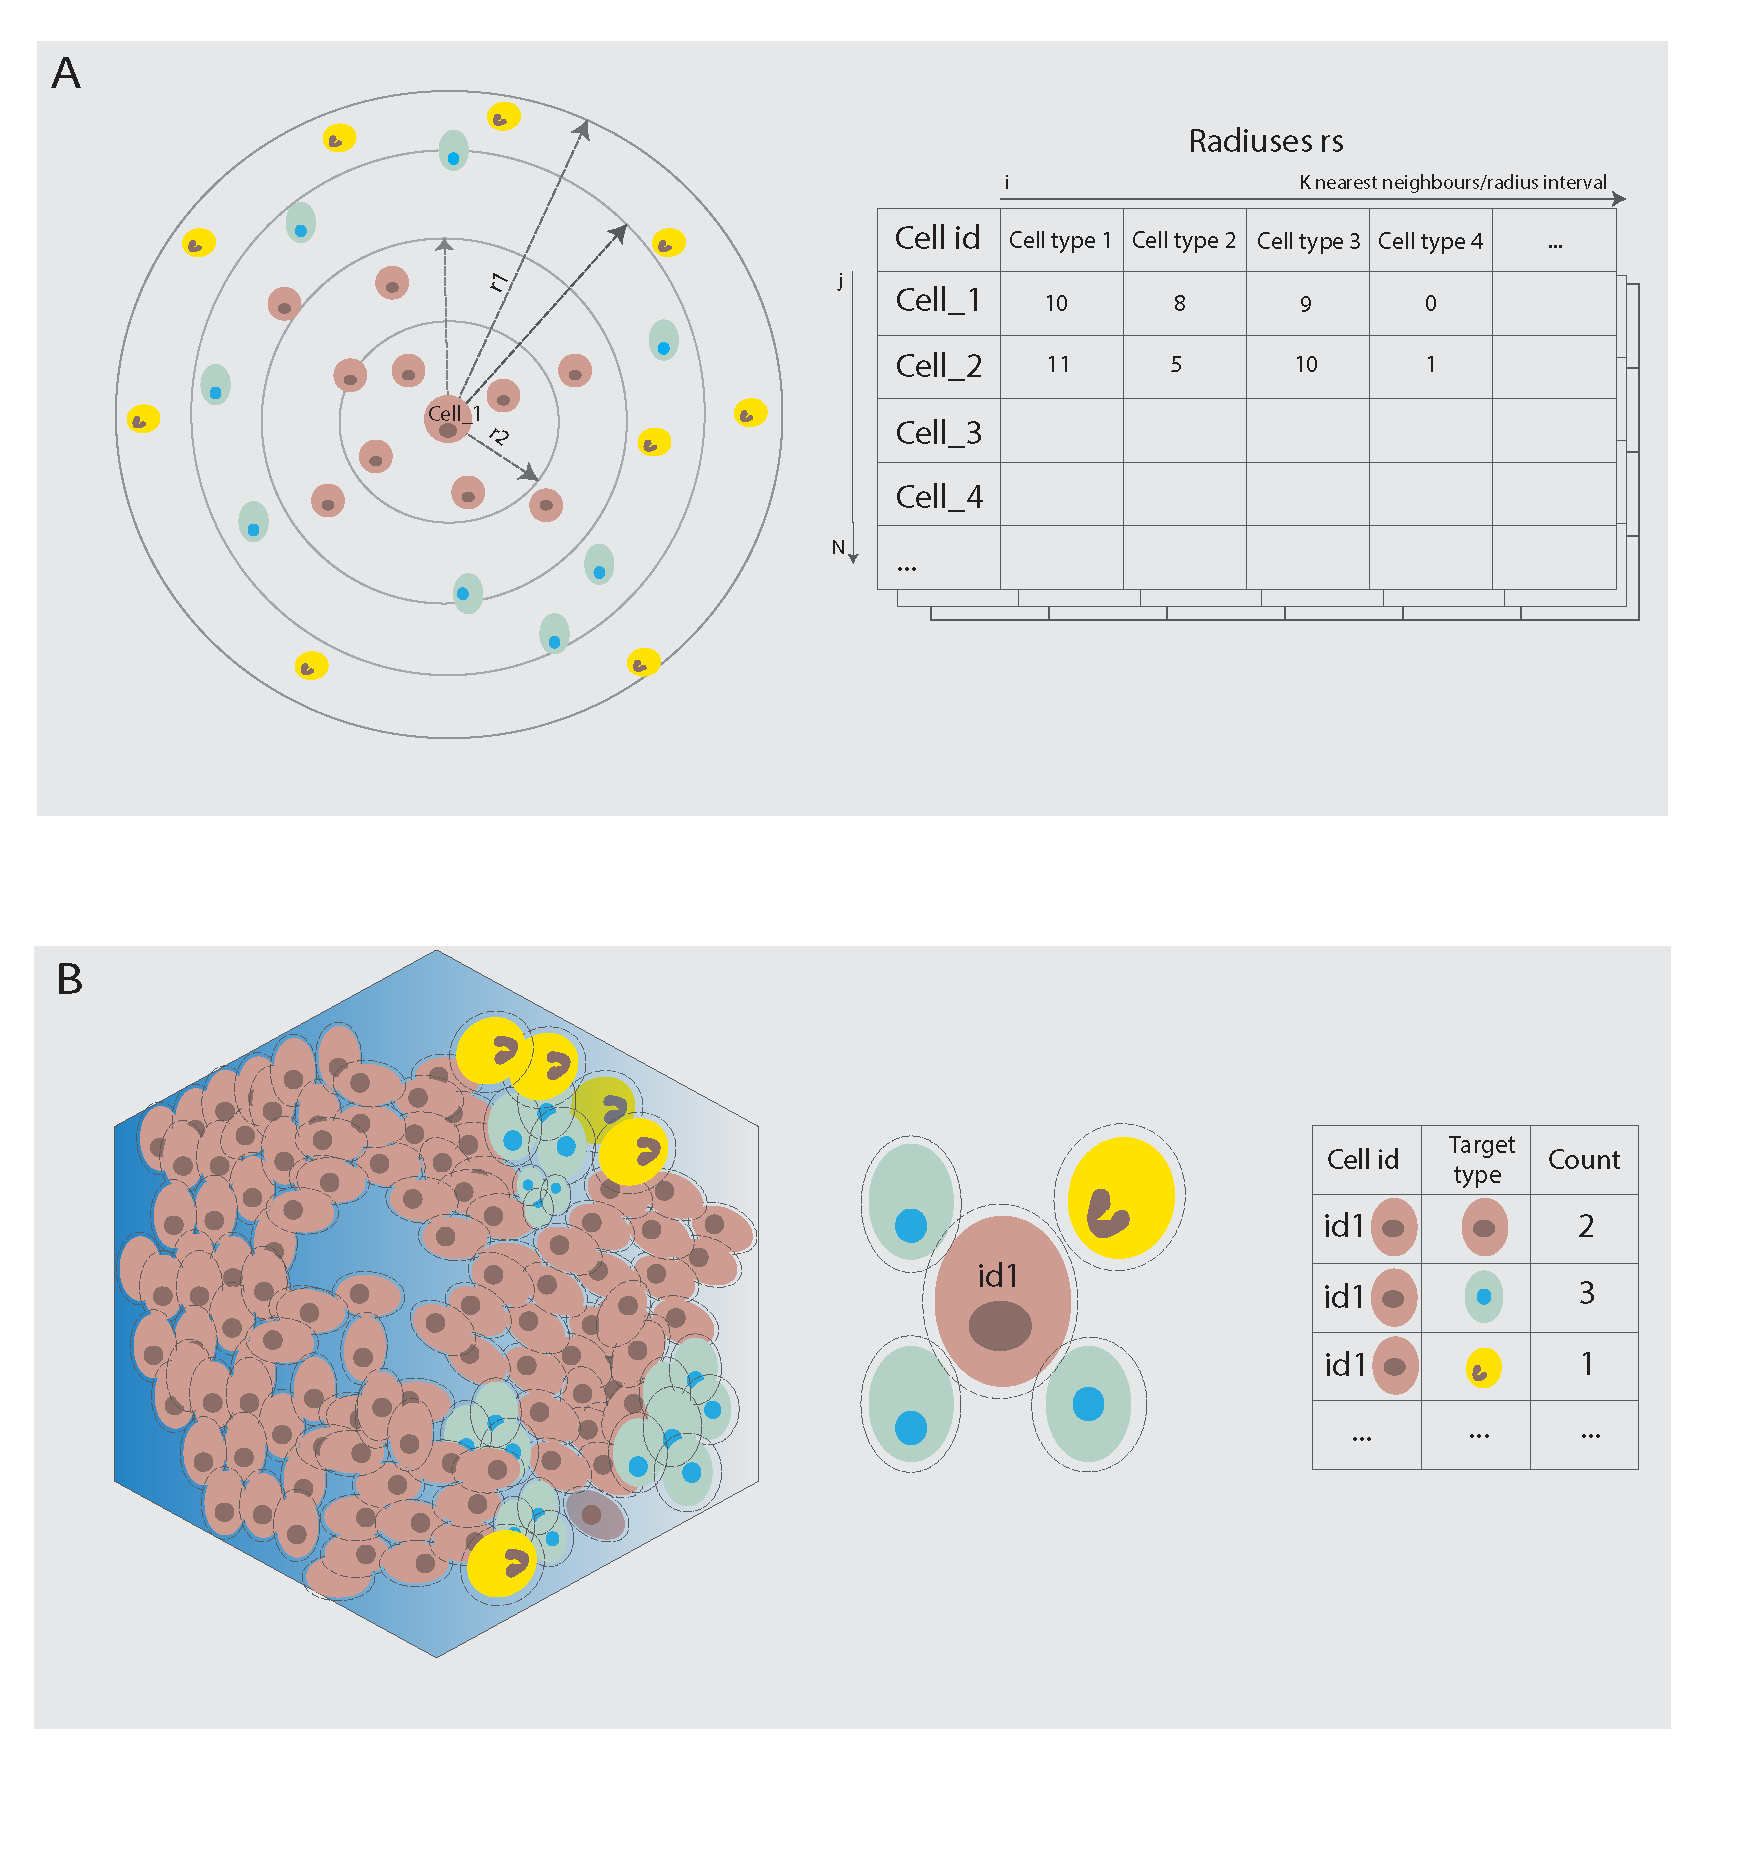
\includegraphics[width=0.85\columnwidth]{Chapter3/Figures/Conceptualise_CCC_analysis_cropped-01.png}
    \caption{Summary of different cell type interaction analyses. (A) Schematic of cell-cell interaction through varied distance interval. The analysis process starts by iterating through every cell then accumulates the information about neighbouring cells to determine the cell spatial identity. (B) Schematic of measuring spatial interaction of cells through counting the number of touching cells. Randomising is applied at the downstream of the analysis to identify the significance of pairwise interaction}
    \label{fig:CCC_conceptualised}
\end{figure}

\subsection{Nearest neighbourhood approach to cells interaction}
% ********* Enter your text below this line: ********
For the second aims of this thesis, I implemented and adopted several methods to uncover the tissue spatial organization by considering each cell as a point process in a 2-dimensional coordinate system. The advantage of this point-process approach is that it can use most of the analytical procedure established in high-level spatial analyses in social studies \cite{yushimito2012voronoi}. It is reasoned that the spatial structure of the tissue is a heterogeneous collection of single cells, consisting of multiple homogeneous groups \cite{schurch2020coordinated}. In this approach, we identify spatial communities throughout the tissue using $K$ nearest neighbour and/or a radial distance approach (Fig: \ref{fig:CCC_conceptualised}A). For each cell across the tissue, the spatial identity of itself is defined by a K number of nearest neighbouring cells (including itself as the reference). The nearest neighbour metric is measured by Euclidean distance between the $X$ and $Y$ coordinates of the cells in the two dimensional tissue section. Alternatively, we can also apply a neighbourhood identification method that is threshold free, known as the Delaunay cell network \cite{guibas1985primitives, dries2021giotto}. The spatial identities of cells are then clustered by their neighbourhood features \ref{fig:CCC_conceptualised}. The clusters of cells based on cell neighbourhood (i.e. spatial identity) can reveal communities of cells within the tissue and the composition of cell type for each community. Such methods have been used and adopted in different fields including eco-geography as well as biology \cite{goltsev2018CODEX, dries2021giotto}.

To ascertain whether cell communities identified by the above approaches followed true spatial patterns, we performed co-occurrence analysis which also employs similar principles as in the nearest neighbourhood approach. This co-occurrence analysis was inspired by an approach introduced by Tosti et al., first applied for spatial transcriptomics data of human pancreas \cite{tosti2021single}. The co-occurrence score can be estimated by the Equation \ref{Eq:Cooc_equation}, which is defined by the fraction of the probability of observing a test cell type $exp$ at the presence of a reference cell type $cond$ ($P_{r}(exp|cond)$) over the probability of observing that test cell type $exp$ $P_{r}(exp)$ at the presence of any other cell type within the same distant interval $r$. At a specific distant $r$, $Co_{r}$ indicates how high/low $exp$ and $cond$ cell types co-localised compared to random cell types. The comparison of $Co_{r}$ at an increasing distant radii $r$ shows how the co-localisation of two cell types starts dispersing.[...]


\begin{align}
\label{Eq:Cooc_equation}
Co_{r} = \frac{P_{r}(exp|cond)}{P_{r}(exp)} 
% K(t) =  \sum_{i=1}^{n}\sum_{n}^{j}1\{d_{ij} < r\} \\ 
\end{align}

For the Polaris skin cancer dataset, we first investigated how different cell types are colocalised into communities using the nearest neighbour approach. By clustering analysis to group regions with similar local density of various cell types, we identified 6 cell communities distributed across the tissue. Quantitative assessment of cell composition in each community allowed us to deduce biologically interpretable features of these communities (Fig: \ref{fig:skin_cancer_polaris}A). Particularly, communities 2 and 3 consisted of scattered immune cells while community 1 appeared to have very high density of epithelial cells positive with PD-L1. This could be explained by the known biological process and tissue structure that cancerous epithelial cells tend to reside densely around the cancer nest, and the presence of immune cells under the epidermis layer (Fig: \ref{fig:skin_cancer_polaris}B,E). On the other hand, clusters 1 and 4 contain mixed epithelial and immune cell populations in the same communities. Comparing the distribution of cell communities and tissue annotation (Fig: \ref{fig:skin_cancer_polaris}B) suggested that the clusters 2, 3 and 4 highly aligned with the stromal microenvironment communities (Fig: \ref{fig:skin_cancer_polaris}D).  Of note, using our own STRISH test (described in more details later), we found spatially-specific interactions between PD1 and PDL1 along the edge of cancer and immune cells \ref{fig:skin_cancer_polaris}C). Furthermore, we investigated the clusters 2 and 3 by co-occurrence analysis (Fig: \ref{fig:skin_cancer_polaris}F). Using T-cells positive with PD1+ protein as the condition (reference) cell type), the co-occurence test confirmed that the co-localisation of these cells with the other two subgroups of T-cells, including double positives CD8+ and FoxP3+ and single positive CD8+ T-cells were higher than random (at distances from $0\mu m$ to $400 \mu m$). Similarly, PanCK+ also co-occured with the CD68+ and PD1+ double positive cluster.       

Applying similar CCC analysis approaches to the colorectal dataset, we sought to test for the co-localization between cancer and immune cells across ROIs. As an example, the general distribution of cells and signals within an ROI is shown in \ref{fig:colorectal_cancer_IMC}A and \ref{fig:colorectal_cancer_IMC}B. Figure \ref{fig:colorectal_cancer_IMC}D shows the probability conditioned on the presence of cancer cells of the ROIs showed in \ref{fig:colorectal_cancer_IMC}A. We could observe a high enrichment of of cancer cells with epithelial cells at the first $200\mu m$ interval. While the co-occurrence analysis could provide insights into how different cell types form cell communities, the analysis is limited to a single ROI at a time. Therefore, we performed an additional analysis where we grouped co-occurrence scores of multiple ROIs together which allowed us to perform Wilcoxon test for the significance of co-localization. The table embedded in the Figure\ref{fig:colorectal_cancer_IMC}E shows the significant test of occurrence scores of between every pair of cell types in our dataset. This new statistical test framework is being developed, and the preliminary results suggested differential cell type co-localisation across patients and should be suitable features to be correlated with clinical outcomes.[...]

\begin{figure}
    \centering
    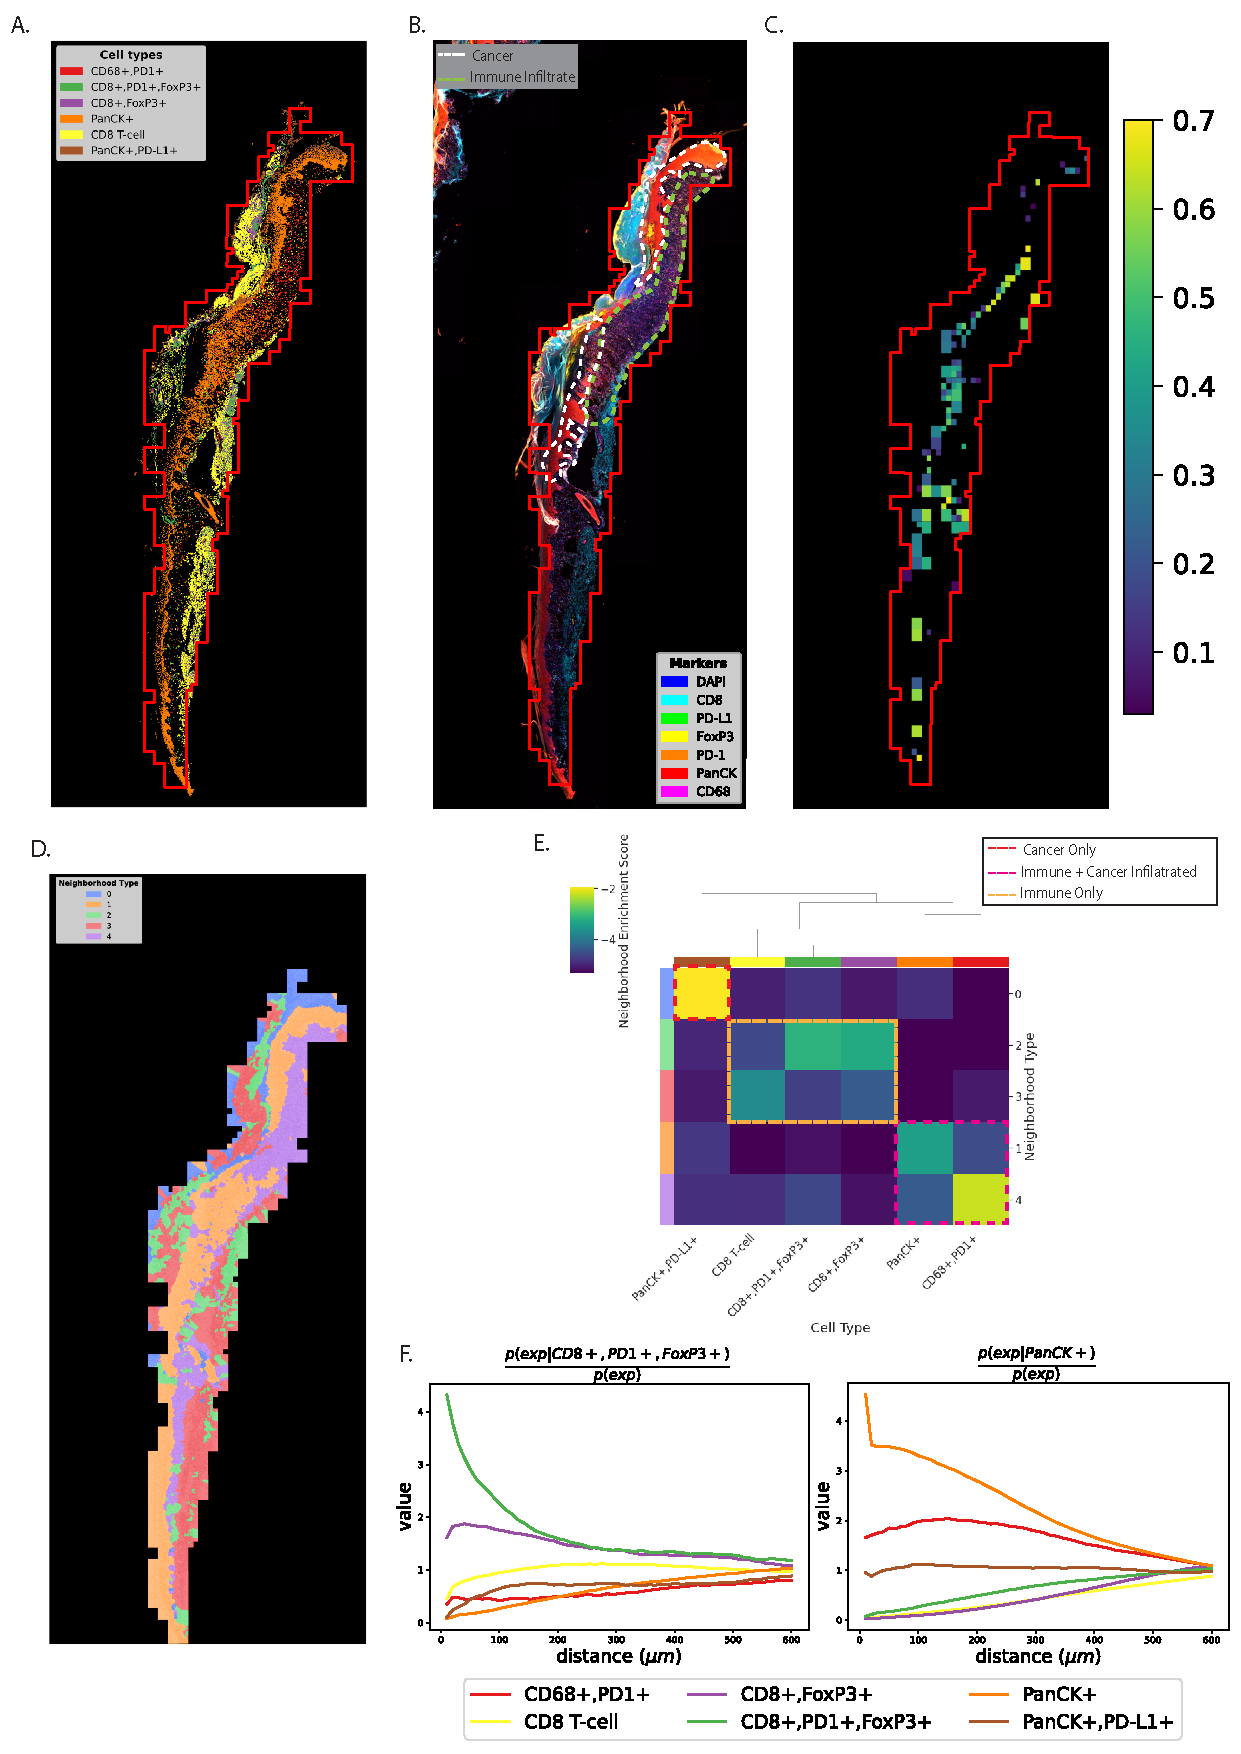
\includegraphics[width=0.8\columnwidth]{Chapter3/Figures/Minh_figure3-01.png}
    \caption{Analyses of Polaris multiplexed imaging of human SCC skin cancer tissue. (A) Cell type classification through clustering and signal gating of the expression of 6 proteins mapped to single cells. The panel of 6 antibodies used to profile the protein expression of major cell types of interest including cytokeratin, cancer secrete immune inhibitor (PD-L1), and immune cells (CD8 T-cell, NK cells, Macrophages). (B) Pathological annotation of cancer and immune regions, based on tissue morphology. (C) Analysis of cancer-immune cell co-localisation through the ligand-receptor pair PD1 and PD-L1. (D) Voronoi which uses the spatial distribution of the cell communities to split the original tissue into multiple regions, representation of distinct cell neighbourhood communities defined via clustering}
    \label{fig:skin_cancer_polaris}
    
\end{figure}
\subsection{A contact-based approach for CCC analysis}
For the colorectal cancer project, we do not have the pathologist annotations for all the ROIs. Therefore, we adopted a slightly different approach to measure near distant CCC. Using the cell segmentation masks as the representation of the cells, we expanded the peripheral of the cell by a margin of 6 pixels and counted the number of touching cells in the adjacent space for pairwise interaction analysis (Figure: \ref{fig:CCC_conceptualised}B). The pairwise interaction was compared to a random distribution using two individual one-tail permutation test within the same image. The test suggested how significant a pairwise interaction between two cell types was compared to random, and eventually suggested an interaction or an avoidance trend. The significance ($P<0.05$) of the contact-based neighbourhood analysis in one of the ROIs shows the most significant interaction starting from epithelial cells toward fibroblast cells. The next significant interactions included those of cancer cells with macrophages and with NK-cells (equally) (Fig: \ref{fig:colorectal_cancer_IMC}C). These results make biological sense and are expected as the cause of colorectal adenocarcinoma are mutated epithelial cells which trigger the growth of surrounding  stromal cells \cite{bremnes2011role}. 

A statistical test to combine the multiple ROIs and tissue sample together for survival prediction and clinical outcome using CCC is also another interesting analysis that I sought to develop and implement on those datasets. Through the multiple spatial methods of cell-cell interaction analyses that I have done so far, I look forward to combining them into a full and comprehensive pipeline for studying CCC with spatial -omic data. This next step is also aligned with my third aim to develop a holistic framework to work with multimodal spatial -omic data and discover different characteristics of CCC throughout cancer tissues. 

% histocat approach which uses the cell outline
\begin{figure}
    \centering
    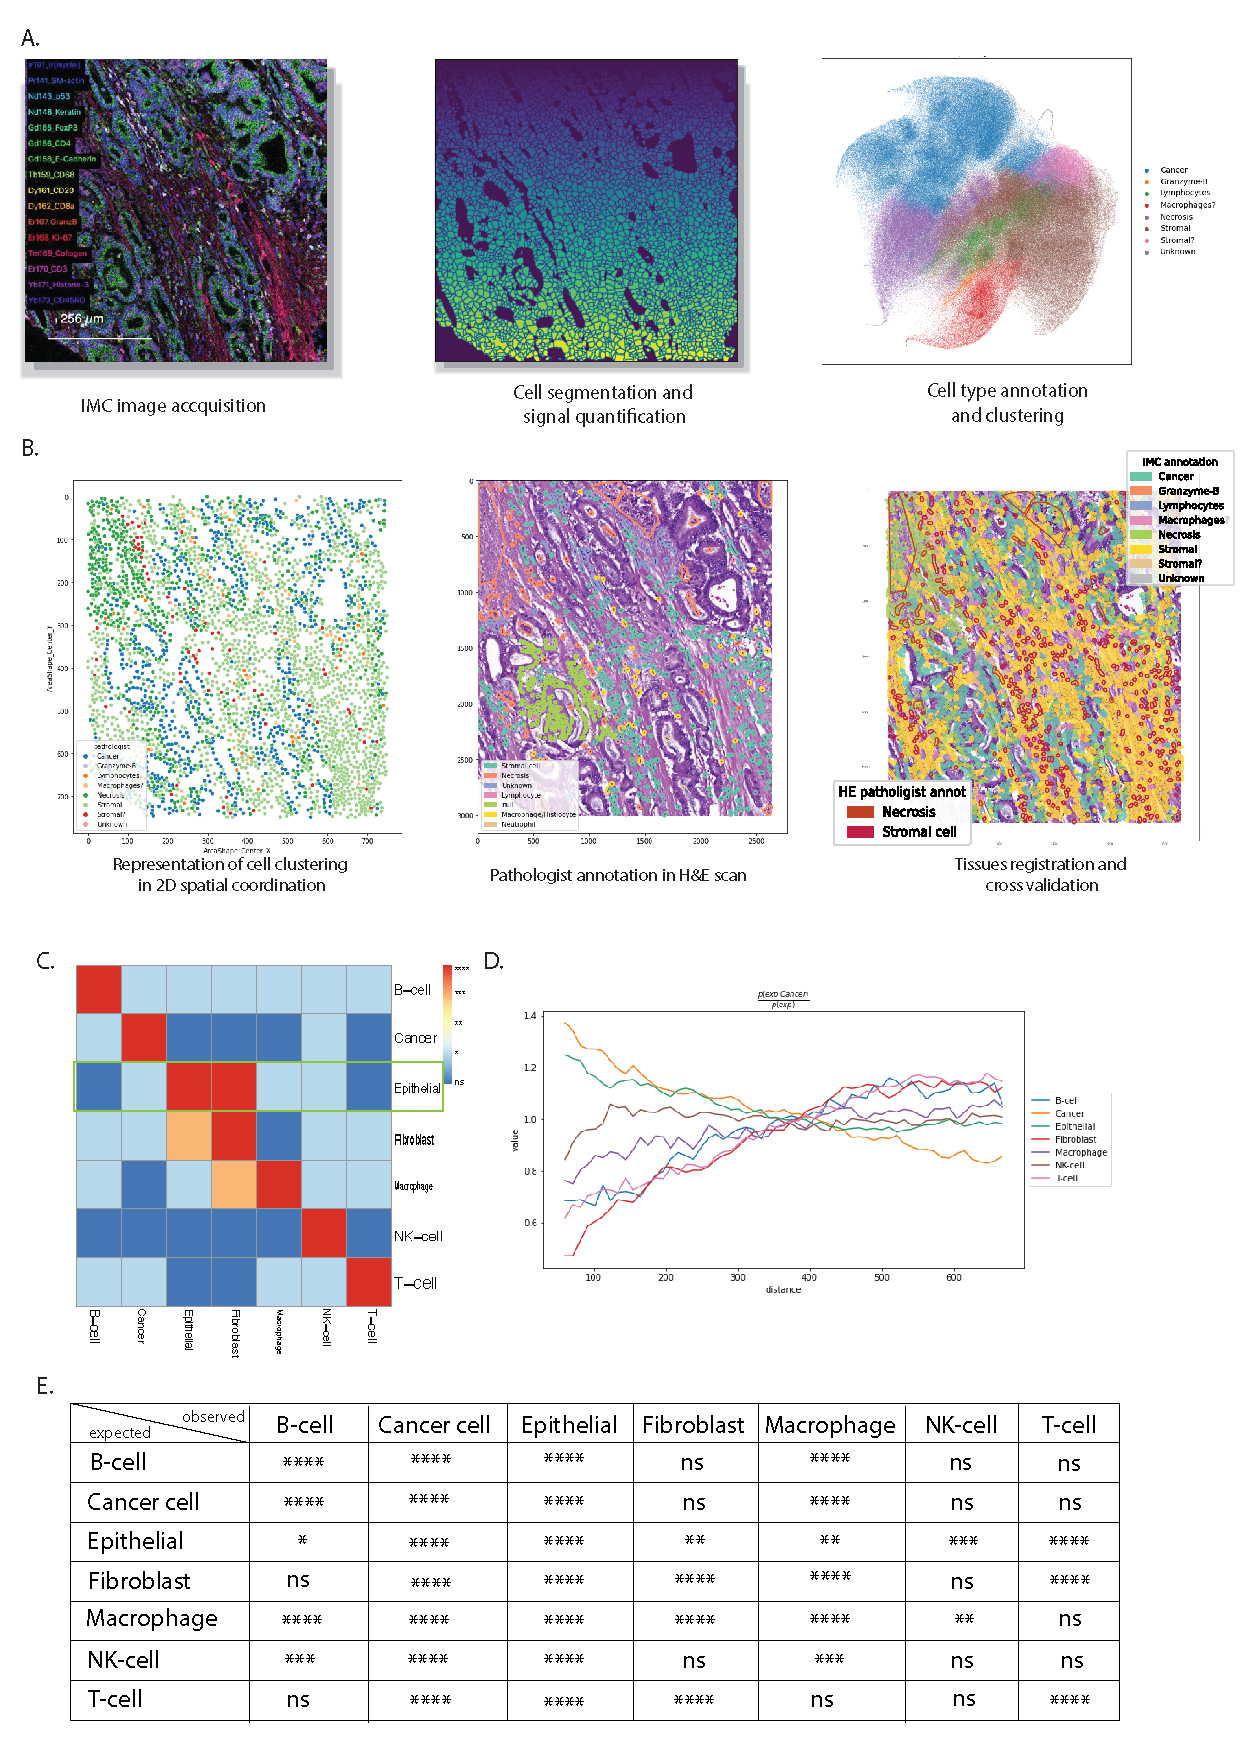
\includegraphics[width=0.8\columnwidth]{Chapter3/Figures/Hyperion_analysis_results-01.png}
    \caption{Keys analysis components of cell type identification and CCC for IMC data. (A) The workflow for the transformation from multiplexed imaging data to non-imaging, single-cell data for clustering pipeline. (B) Visualization of cell type annotation and validation against pathologist H\&E annotation. (C) The landscape of intercellular communication across a sub-sample of the whole IMC dataset. (D) An example of co-occurrence analysis of different cell types in the presence of cancer cells at increasing distance thresholds. (E) A summary of significance co-occurrence score across all combinations of observed and expected cell types.}
    \label{fig:colorectal_cancer_IMC}
    
\end{figure}
% ***************************************************
\section{STRISH for cell co-localisation with spatial proteomic data}
\label{Sec:3.3_STRISH2.0}	%CREATE YOUR OWN LABEL.
Spatial information at the subcellular level can facilitate a lower level of spatial analysis, which uses the cell geometry and density to assist the interaction analysis. As described before, in the Polaris dataset, we scanned all the regions, where cancer and immune cells co-localised and interacted via PD-L1 and PD1. Using the cell clustering information, I developed and applied a STRISH scanning window strategy to search for regions where there are immune cells double positive for CD8+ and PD1+ in the immediate vicinity of cancerous epithelial cells (which themselves are double positive for PanCK+ and PD-L1+). The STRISH scanning window strategy starts with a broad scale (i.e 4 non-overlapped tiles at the size of of one fourth of the original slide scan) and gradually splits large tiles into smaller windows until a cell-count threshold is met (less than 100 cell per windows by default). Subsequently, the results from cell detection are scored, normalised and used to plot a heatmap for localised regions (neighbourhood) with co-localisation of the two cell types being tested. Figure \ref{fig:skin_cancer_polaris}C shows the activity map of CD8+, PD1+ cells and PanCK+, PD-L1+ cells throughout the tissue. Interestingly, these two cell types were mostly observed to be co-localised at the interface of cancer and immune infiltration, according to the pathologist's annotation. The heatmap provided visual and quantitative evidence of CCC occurring between cells in our tissue sample. This analysis result is being integrated in a multimodal project to create atlas of skin cancer and cell-cell interaction with other 5 complementary technologies (manuscript under preparation).

Regardless of the input datatype, all the multiplexed imaging technologies, which captured the transcript or protein expression at subcellular level, can be processed by a similar workflow. Collectively, the data processing should include data transformation into standard multidimensional image data, cell segmentation, and signal mapping for each staining channel \cite{shakya2020immune, liu2019comparison, aghaeepour2013critical}. In this thesis, I first developed a pipeline for RNAscope data and then extended to various types of spatial omic data. I made some major refactors to the STRISH pipeline in the past year to make it a more versatile framework. 
As mentioned above, after a standard data preprocessing, the resulting multidimensional image is converted into a single-cell data matrix. A set of new functions for data loading to STRISH are added, so that STRISH object can interact with an Anndata object \cite{wolf2018scanpy} to take advantage of this data object structure commonly used for single-cell matrices. Additional spatial coordination information is included in the object. This approach allows us to customise the object while still making use of various methods of single cell data normalisation and clustering methods. 

For CCC analysis, STRISH introduces a new method for cell co-localisation detection through windows scanning. STRISH identifies whether there are cells that expressing compatible ligands and receptors that locate within the window(local microenvironment) and summarised the results in an interpretable heatmap. As the tissue fluorescence image contain gaps between cells this makes tissue segmentation a challenging task. In STRISH, it is possible to use the scanning windows to accommodate for these gaps for calculating co-localisation. STRISH generates tissue contour to highlight the tissue region from the background. Several recent analysis features include automated cell segmentation and cell type clustering integrated with spatial information; nearest neighbourhood and co-occurrence approaches are also included in the framework. Finally, to increase the adaptability of multimodal analysis, image registration to align two tissue images from different rounds of experiments with minor variations is also included.   

It is important to acknowledge that STRISH particularly focuses on CCC analyses in spatial transcriptomic and proteomic data. Hence, it should not be used in isolation but in combination with other data normalisation and cell type clustering tools. Existing tools such as Giotto and Squidpy also provide multiple functions for spatial analysis and interactive graphical user interface. While such features are useful for exploratory analysis, STRISH features are tailored to cell-cell interaction through ligand-receptor and multimodal data analysis. To improve STRISH, I also seek to introduce more statistical tests and spatial quantitative measurement into the current pipeline.

\section{Quantitative and qualitative measurement}
\label{Sec:3.4_validation}	%CREATE YOUR OWN LABEL.
\subsection{Spatially differential analysis across images}

\subsection{Correlation of spatial organisation to clinical survival rate}

\label{Sec:4.2_CCC_in_COAD}	%CREATE YOUR OWN LABEL.
\subsection{Cell type community and heterogeneity in cancer tissues}
% ********* Enter your text below this line: ********
We introduce 

% ********* Enter your text below this line: ********
By aggregating cell's neihgborhood from multiple ROIs, STRISH allows the spatial differential analysis across the  conditions and uncover the relationship between treatment outcome and spatial organisation of cell types.



% ***************************************************
% \bibliographystyle{elsarticle-num}

% \bibliography{./References/Bibliography}